% !TEX encoding = UTF-8
% !TEX TS-program = pdflatex
% !TEX root = ../tesi.tex
% !TEX spellcheck = it-IT

%**************************************************************
\chapter{Progettazione e codifica}
\label{cap:progettazione-codifica}
%**************************************************************

\intro{Breve introduzione al capitolo}\\

%**************************************************************

\section{Angular MVC}
AngularJS è stato il framework maggiormente utilizzato in questo stage e mi ha consentito di implementare l'intero progetto agilmente.\\
Alla base del framework, è collocato il design pattern \gls{mvc}, leggermente modificato per adattarsi alle funzionalità di AngularJS. Il design pattern che ne risulta è qualcosa di più flessibile del classico \gls{mvc}, consentendo agli sviluppatori una maggior libertà di utilizzo.\\
Ovviamente ci sono delle direttive e delle best practice consigliate, soprattutto se si intende creare un \gls{frontend} davvero \gls{rest}-ful.

\subsection{Two-way Data Binding}
Una funzionalità importante che AngularJS espone è il cosiddetto \emph{Two Way Data Binding}. Si parla di \emph{legame doppio tra dati} quando una variabile del modello è legata ad un elemento che può cambiare ed al contempo mostrare il contenuto della variabile stessa. In una vista di AngularJS, ogniqualvolta un elemento che applica il \emph{Two Way Data Binding} viene modificato, il corrispondente campo nel modello viene notificato e aggiornato correttamente.\\
In AngularJS, si usa la direttiva \textbf{ng-model} per legare una variabile del modello ad un elemento \gls{html} che può sia mostrare il suo valore, che modificarlo.

\begin{figure}[H] 
    \centering 
    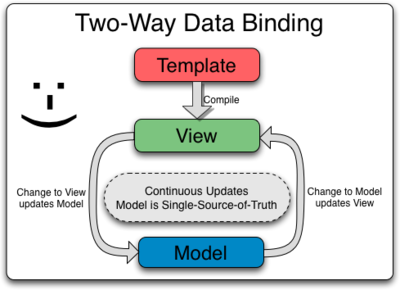
\includegraphics[width=0.8\columnwidth]{two_way_data_binding} 
    \caption{Doppio legame tra vista e modello di AngularJS}
\end{figure}




%**************************************************************

\section{Stub Backend}
Il progetto di stage ha avuto come oggetto la realizzazione di un \gls{frontend} gestionale, senza però avere al contempo un \gls{backend} funzionante. Per le verifiche funzionali, quindi, ho avuto bisogno di realizzare un \gls{backend} fittizio, il quale mi consentisse di effettuare chiamate alle \gls{api} concordate con il Responsabile di Progetto per il backend vero e proprio.\\
Per realizzare questo \gls{backend} sono ricorso a delle feature fornite dalle librerie di AngularJS adibite al testing di unità. Durante il testing delle funzionalità di una componente, le richieste ad un server funzionante vengono sostituite con una chiamata ad hoc che deve rispettare certe precondizioni e che restituisce dei dati prestabiliti. Il concetto del \gls{backend} di \gls{stub} che ho utilizzato è lo stesso. In particolare, grazie all'utilizzo di espressioni regolari per filtrare le chiamate \gls{rest}, sono stato in grado di intercettare tali chiamate e di farle gestire al mio \gls{backend} ad hoc, con risposte prestabilite.\\
Tutto ciò è stato possibile gran parte grazie al servizio \textbf{\$httpBackend} di AngularJS, il quale contiene metodi di intercettazione di chiamate \gls{rest} e di gestione di richieste e risposte \gls{http}. Il frammento sottostante è un esempio di una chiamata \gls{http} gestita dal \gls{backend} di \gls{stub}:

\begin{verbatim}
$httpBackend.whenGET(/\/api\/\d.\d\/users\/\w*\/qualification/).respond(function(method, url, data, headers) {
  console.log('Received these data:', method, url, data, headers);
  var getStatus,
   getData = {},
   getHeaders = headers;
  if(headers.Authorization == "Bearer XXX") {
    getStatus = 200;
    getData = {
      qualifications: [
        {
          type: 'Workshop',
          authority: 'W3C',
          address: 'Silicon Valley, 42',
          grade: 'Senior',
          earnDate: new Date(2015, 4, 20).toISOString(),
          vendor: 'RFC',
          product: 'HTML6',
          expireDate: new Date(2050, 4, 20).toISOString()
        },
        {
          type: 'Certificazione',
          authority: 'Mongo',
          address: 'MongoDB avenue, 8080',
          grade: 'Senior',
          earnDate: new Date(2014, 7, 8).toISOString()
        },
        {
          type: 'Corso',
          authority: 'AngularJS',
          address: '1600 Amphitheatre Parkway Mountain View, CA 94043',
          grade: 'Junior',
          earnDate: new Date(2015, 5, 20).toISOString()
        }
      ]
    };
  }
  else
    getStatus = 401;
  return [getStatus, getData, getHeaders];
});
\end{verbatim} 

%**************************************************************

\section{Tecnologie e strumenti}
\label{sec:tecnologie-strumenti}

Di seguito viene data una panoramica delle tecnologie e strumenti utilizzati.

\subsection*{Tecnologia 1}
Descrizione Tecnologia 1.

\subsection*{Tecnologia 2}
Descrizione Tecnologia 2

%**************************************************************
\section{Ciclo di vita del software}
\label{sec:ciclo-vita-software}

%**************************************************************
\section{Progettazione}
\label{sec:progettazione}

\subsubsection{Namespace 1} %**************************
Descrizione namespace 1.

\begin{namespacedesc}
    \classdesc{Classe 1}{Descrizione classe 1}
    \classdesc{Classe 2}{Descrizione classe 2}
\end{namespacedesc}


%**************************************************************
\section{Design Pattern utilizzati}

%**************************************************************
\section{Codifica}
